\documentclass[border=8pt,tikz]{standalone}
\usepackage{tikz}
% Shared TikZ style for Chapter 5 diagrams.
% Inputted by every standalone diagram file.

\usetikzlibrary{
  arrows.meta,
  positioning,
  shapes.geometric,
  shapes.symbols,
  shapes.multipart,
  shapes.misc,
  fit,
  calc,
  backgrounds,
  decorations.pathmorphing,
  decorations.pathreplacing,
  patterns,
  shadows.blur,
}

% ─── Colour palette ──────────────────────────────────────────────
\definecolor{strixBlue}{HTML}{3B7DD8}     % data sources / inputs
\definecolor{strixGreen}{HTML}{22A699}    % processing / workers
\definecolor{strixOrange}{HTML}{E08036}   % storage
\definecolor{strixRed}{HTML}{E04B4B}      % attacker / external threat
\definecolor{strixPurple}{HTML}{6B5DD3}   % frontend / UI
\definecolor{strixGold}{HTML}{F2BE22}     % models / ML
\definecolor{strixGrey}{HTML}{6E7681}     % neutral / labels
\definecolor{strixDark}{HTML}{1F2933}     % titles / borders

% ─── Common node styles ──────────────────────────────────────────
\tikzset{
  >={Latex[width=2mm,length=2.5mm]},
  font=\sffamily\small,
  every node/.style={align=center},
  comp/.style={
    rectangle, rounded corners=2pt, draw=#1, fill=#1!10, very thick,
    text=strixDark, minimum width=22mm, minimum height=8mm,
    inner sep=4pt,
  },
  comp/.default=strixGreen,
  store/.style={
    cylinder, shape border rotate=90, aspect=0.3, draw=strixOrange,
    fill=strixOrange!12, very thick, text=strixDark,
    minimum width=18mm, minimum height=10mm, inner sep=2pt,
  },
  stream/.style={
    rectangle, rounded corners=2pt, draw=strixOrange,
    fill=strixOrange!8, dashed, thick, text=strixDark,
    minimum width=22mm, minimum height=7mm, inner sep=3pt,
    font=\ttfamily\scriptsize,
  },
  source/.style={comp=strixBlue},
  worker/.style={comp=strixGreen},
  model/.style={comp=strixGold},
  ui/.style={comp=strixPurple},
  ext/.style={comp=strixRed},
  title/.style={font=\sffamily\bfseries, text=strixDark},
  edge/.style={->, thick, draw=strixGrey, font=\sffamily\scriptsize\itshape},
  edgeStrong/.style={->, very thick, draw=strixDark, font=\sffamily\scriptsize\bfseries},
  group/.style={
    rectangle, rounded corners=4pt, draw=strixGrey, dashed, thick,
    inner sep=6pt, fill=strixGrey!4,
  },
  badge/.style={
    rectangle, rounded corners=1pt, fill=#1, text=white,
    font=\sffamily\scriptsize\bfseries, inner sep=2pt,
  },
  badge/.default=strixDark,
  port/.style={
    rectangle, rounded corners=1pt, draw=strixDark, fill=strixGrey!8,
    font=\ttfamily\scriptsize, minimum width=14mm, inner sep=2pt,
  },
}


\begin{document}
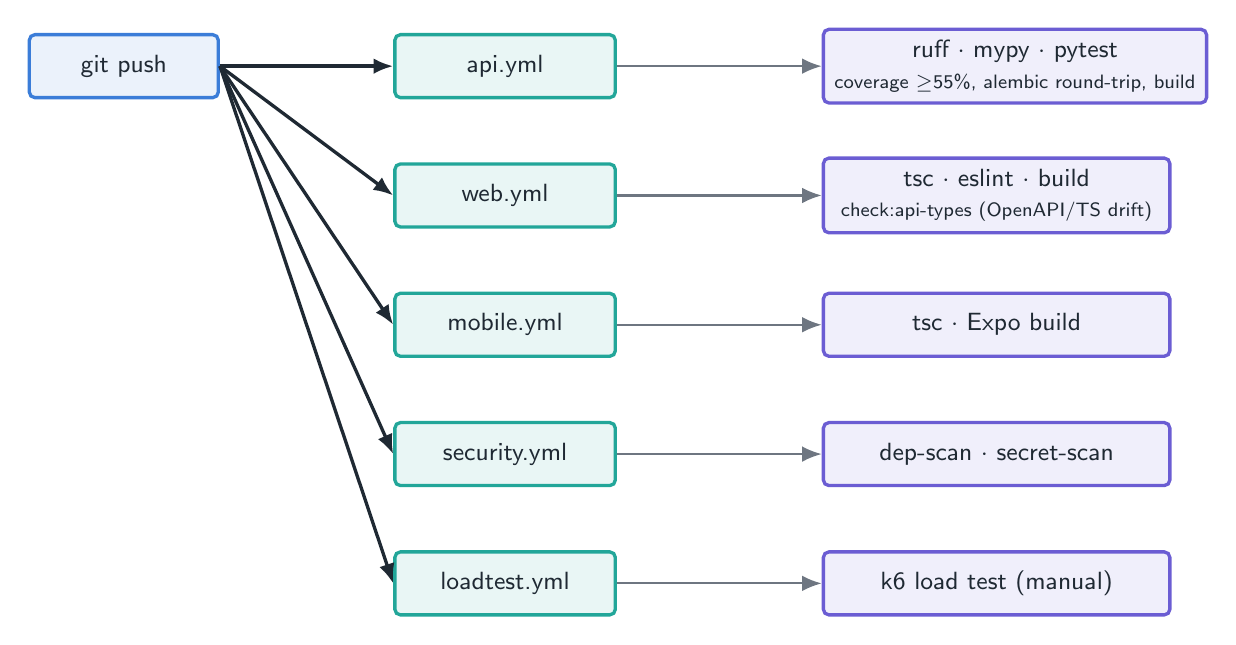
\begin{tikzpicture}[node distance=6mm and 14mm]

\node[source, minimum width=24mm] (push) {git push};

\node[worker, right=22mm of push, minimum width=28mm] (api) {api.yml};
\node[worker, below=8mm of api, minimum width=28mm] (web) {web.yml};
\node[worker, below=8mm of web, minimum width=28mm] (mob) {mobile.yml};
\node[worker, below=8mm of mob, minimum width=28mm] (sec) {security.yml};
\node[worker, below=8mm of sec, minimum width=28mm] (lt)  {loadtest.yml};

\node[ui, right=26mm of api,minimum width=44mm] (a1) {ruff \(\cdot\) mypy \(\cdot\) pytest\\\scriptsize{coverage \(\geq\)55\%}, alembic round-trip, build};
\node[ui, right=26mm of web,minimum width=44mm] (a2) {tsc \(\cdot\) eslint \(\cdot\) build\\\scriptsize check:api-types (OpenAPI/TS drift)};
\node[ui, right=26mm of mob,minimum width=44mm] (a3) {tsc \(\cdot\) Expo build};
\node[ui, right=26mm of sec,minimum width=44mm] (a4) {dep-scan \(\cdot\) secret-scan};
\node[ui, right=26mm of lt, minimum width=44mm] (a5) {k6 load test (manual)};

\foreach \w in {api,web,mob,sec,lt} {
  \draw[edgeStrong] (push.east) to[bend left=0] (\w.west);
}
\foreach \src/\tgt in {api/a1,web/a2,mob/a3,sec/a4,lt/a5} {
  \draw[edge] (\src) -- (\tgt);
}

\end{tikzpicture}
\end{document}
